\documentclass[12pt]{article}

% Packages
\usepackage[a4paper, margin=1in]{geometry} % Adjust margins
\usepackage{setspace} % For line spacing
\usepackage{tocloft} % Optional: better spacing for TOC
\usepackage[backend=biber,style=apa]{biblatex} % Load biblatex with APA style
%these packages I need for the table
\usepackage{booktabs}
\usepackage{threeparttable}
\usepackage{caption}
\usepackage{geometry}
\usepackage{graphicx}   % Required for including images
\geometry{margin=1in}

\addbibresource{references.bib} % Link to your .bib file

% Set line spacing
\onehalfspacing % or use \doublespacing for double spacing

% Title information
\title{\textbf{\large{Preferences on Tax Enforcement and Tax Administration}}}
\author{\normalsize{Tim Kircali, Stefanie Stantcheva, Matthias Weber}}
\date{\normalsize{30.04.2025}}
\begin{document}
\maketitle
\pagenumbering{arabic}
\begin{center}
    \textbf{Quick note on relevant data in the US tax system}
\end{center}
\tk{I have to dig much more into which exact policies our comprehensive third party reporting policy would include}
\section{Current State of Information Exchange}
A key point of our analysis is to understand what data the US tax administration currently holds, what data it needs and when it needs it to fulfil its services.  More specifically, we want to understand what data is required for two distinct purposes: 1) To detect and prevent tax evasion for tax enforcement purposes. 2) To potentially fulfil tax filing services for taxpayers, such as prepopulating tax returns. 
\subsection{Data to tax enforce:} 
Looking at details of the tax gap (see Table 1), underreporting is mainly the problem of the individual income tax (68\%) and the employment tax (21\%) . A Gao Report (GAO-19-558T Tax Gap) further evaluates: "Individual income taxes made up the largest portion (\$264 billion) of underreporting. Underreporting of business income accounted for nearly half (\$125 billion) of that amount" and "business income underreporting includes income from sole proprietors, which accounted for the largest share (\$78 billion) of individual income tax underreporting". 
The most relevant positions in underreporting are also those where information reporting is poor or non-existent (GAO-19-558T Tax Gap): "For example, according to 2008–2010 IRS data, taxpayers misreported more than half of the types of income for which there is little or no third-party information reporting, such as business income" (see Figure 1). \\
The greatest potential for reducing tax evasion through third-party reporting lies in introducing more information reporting in the following areas:
\begin{itemize}
    \item Tax relevant data where little or no third party reporting exists: Sale of business property, sole proprietor income, rents and royalities, farming income/loss, other non business non-business income
    \item Tax relevant data where some third party reporting exists: Income from partnerships, S corporations, Estate and trusts, Alimony, capital gains. 
\end{itemize}

\begin{table}[htbp]
\centering
\caption{Estimated Average Annual Individual Income Underreporting Tax Gap by Tax Return Item or Category, Tax Years 2008 to 2010\\
(Dollars in billions), Source: GAO-19-558T}
\begin{threeparttable}
\begin{tabular}{@{}llr@{}}
\toprule
\textbf{Tax return items or category} & & \textbf{Tax gap estimate} \\ 
\midrule
\textbf{Business income} & & \textbf{125} \\
\quad Sole proprietor income & & 78 \\
\quad Income from partnerships, S corporations, estates/trusts & & 22 \\
\quad Rents and royalties & & 20 \\
\quad Farming income/loss & & 5 \\[2pt]
\textbf{Non-business income} & & \textbf{64} \\
\quad Other income\tnote{a} & & 29 \\
\quad Capital gains & & 11 \\
\quad Taxable Social Security benefits & & 7 \\
\quad Pensions and annuities & & 5 \\
\quad Wages & & 5 \\
\quad Business sale/Form 4797 income & & 4 \\
\quad Dividends & & 1 \\
\quad Interest & & 1 \\
\quad State income tax refunds & & 1 \\
\quad Unemployment compensation & & 1 \\[2pt]
\textbf{Credits} & & \textbf{40} \\
\quad Earned income tax credit & & 27 \\
\quad Child tax credit & & 7 \\
\quad Education credits & & 4 \\
\quad Other credits & & 2 \\[2pt]
\textbf{Deductions} & & \textbf{18} \\
\quad Unallocated marginal effects \tnote{b} & & 12 \\
\quad Exemptions & & 6 \\
\quad Filing status & & 5 \\
\quad Other taxes & & 1 \\
\quad Adjustments\tnote{c} & & -5 \\[4pt]
\textbf{Total individual income underreporting} & & \textbf{264} \\
\bottomrule
\end{tabular}
\begin{tablenotes}
\item[a] Includes alimony, gambling, prizes, and other miscellaneous income.
\item[b] Reflects interactions among items that affect total underreporting.
\item[c] Includes adjustments for self-employment tax and other corrections.
\end{tablenotes}
\end{threeparttable}
\end{table}
\begin{figure}[htbp]
\centering
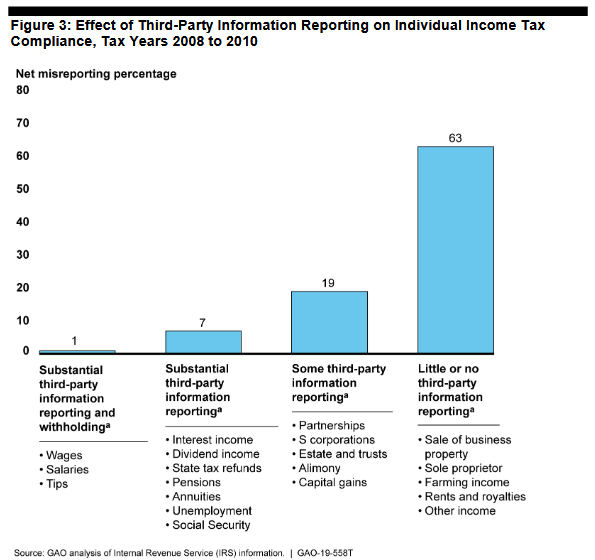
\includegraphics[width=0.85\textwidth]{Figures_Notes/ThirdPartyReporting_Evasion.png}
\caption{Source: GAO-19-558T}
\label{fig:thirdparty_evasion}
\end{figure}
\subsection{Data to prepopulate} 
And how would the IRS be able to prepopulate? Firstly, the IRS already has access to a lot of relevant data, but this data is not processed before the deadline for submitting individual tax returns. The GAO (GAO-21-102) evaluated that 'two factors contribute significantly to returns being processed after the deadline: (1) extensions available to third parties that submit information returns and (2) capacity issues in IRS legacy systems processing the returns. It is of key importance for the IRS to have processed all available tax-relevant data in order to offer prepopulated tax returns.

\begin{figure}[htbp]
\centering
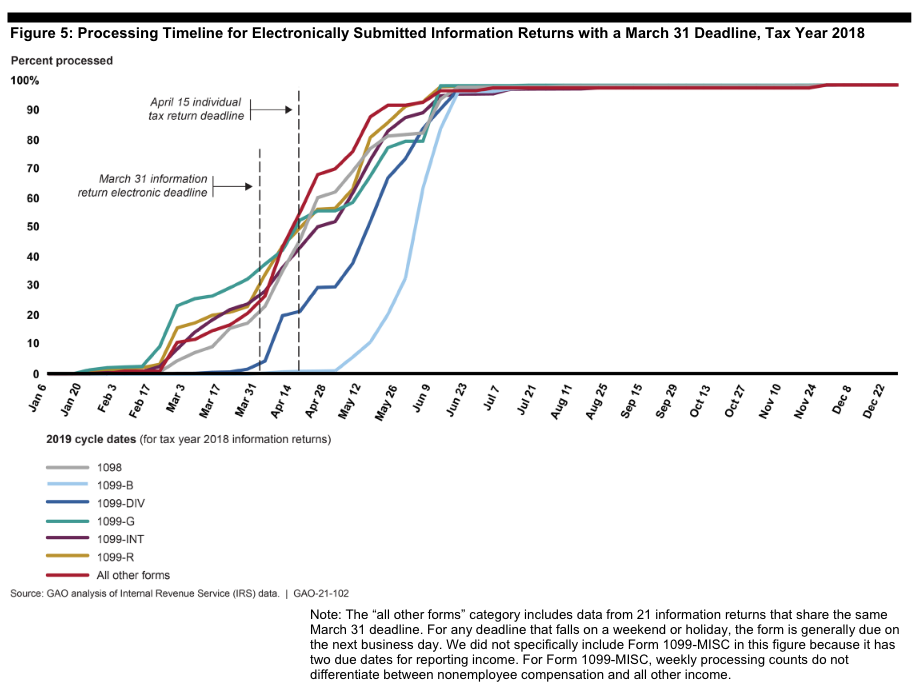
\includegraphics[width=0.85\textwidth]{Figures_Notes/IRS_DataProcessing.png}
\caption{Source: GAO-21-102}
\label{fig:thirdparty_evasion}
\end{figure}

Second, the IRS might not have the relevant data (for all taxpayers). \cite{goodman2023automated} "check for tax situations that would result in an inaccurate prepopulated return, such as reporting a nontrivial amount of income, deduction, or credit on the 2019 filed tax return that the IRS does not observe on an information return" and they find that 48\% of tax returns could be successfully prefilled.\footnote{They make the strong assumption that the IRS already holds all the information at the point of prepopulating, which is not the case, as described above.} And "among the 52 percent of taxpayers who fail the item-based approach, the majority have only one failure situation. Such taxpayers would typically need to make only one change or complete one additional schedule (e.g., reporting self-employment income and deductions on Schedule C — and attaching any schedules required for that Schedule C which would be the most common edit required) to correct their prepopulated return."

They evaluate that "the failure situations fall into three sets. 1) The first set includes those situations where the tax-unit composition changed — for example, a baby is born, or the taxpayer married or divorced. 2) The second set includes situations where the taxpayer claims a tax credit or deduction that is not covered by information returns. This includes essentially everyone who itemizes their deductions, as there is no information return for state property taxes or charitable contributions, which (together) are nearly universal among itemizers. 3) The third set includes situations where the taxpayer has income that either is unreported on information returns or does not match (subject to a tolerance threshold) the income based on information returns. For example, a failure situation occurs when Schedule C (sole proprietorship) net income does not match nonemployee compensation from Form 1099-MISC, which can occur if a taxpayer has other self-employment income or has expenses to deduct. In total, we identify 22 failure situations."

\begin{enumerate}
    \item The first set of situations could be addressed with better information about the tax unit composition. 
    \begin{itemize}
        \item Does another government institution have this data, and could it be potentially exchanged?
        \item Another option would be for the IRS to obtain this information through personal validation of prepopulated returns by asking respondents whether the information had changed. 
    \end{itemize}
    \item It is interesting to approach the second one because some government entities already have data, but this is not being exchanged with the IRS. Some relevant deductions examples where the IRS has not full access to data is:  
    \begin{itemize}
        \item State income tax: is collected at state level, is not directly transmitted to the IRS and is deductible. But the IRS has indirect (partial) information through W2 forms. 
        \item Local income tax: is collected at the city/county. But the IRS has indirect (partial) information through W2 forms. 
        \item Property tax: the local government has information but this is not exchanged with IRS. 
        \item Sales tax: the IRS doesn’t see your purchases or sales tax paid; only relevant if you claim the optional deduction instead of state income tax.
        \item Charitable contributions: Deductible if itemized, but you must self-report; IRS can only audit with receipts.
        \item Childcare expenses: Needed for tax credits, but not automatically reported.
        \item Medical expenses:
        \item State tuition or education payments:
        \item note: Medicaid is not deductable or tax relevant. but having medicaid is tax relevant. Because you then are eligible for premium tax credit.
\end{itemize}
    \item Addressing the third set of information might need the same data the IRS needs to better enforce (as described above.)
\end{enumerate}

\subsection{Specific Policy Proposals}
\subsubsection{To reduce domestic tax evasion}
The greatest potential to reduce the tax gap stems from taxpayers' business income sources, namely from sole propriotorship, partnerships, S corporations, estates/trusts, rents/royalties. A policy that focuses on this group would be beneficial.

The U.S. Government Accountability Office (GAO) has recommended that the IRS research and evaluate potential ways to expand third-party reporting to better capture income and expenses of sole proprietors, a major tax gap category. The IRS was studying this but had not formalized a proposal as of mid-2025. But: Proposals/Ideas to expand third-party reporting for sole proprietors generally focus on requiring platforms, business payers, or financial institutions—rather than individual consumers—to report annual gross receipts, thereby increasing verification while avoiding transaction-level monitoring.

The main idea of existing policies is that someone has to third-party report (to the IRS) payments made to sole proprietors. There is already something in place where businesses above certain payment thresholds have to report to the IRS. Important to note is that end-consumers do not have to report. If payment goes through a platform (PayPal, Uber, Etsy, etc.) then the platform might also have to report (there are some thresholds and exemptions). These thresholds and exemptions have been changed under Biden and back again under Trump. 

Another option would be the idea of aggregate bank-flow reporting. Banks would report inflows and outflows for all bank accounts above a certain low threshold: This was originally proposed in 2021\footnote{\url{https://home.treasury.gov/news/press-releases/jy0415}, \url{https://www.bakerbotts.com/thought-leadership/publications/2021/may/us-treasury-publishes-plan-to-close-the-tax-gap-and-raise-700-billion}} but led to huge privacy backslash\footnote{\url{https://edition.cnn.com/2021/10/08/politics/irs-spying-600-republicans-fact-check}}. Now discussions are going on for weaker versions of the initial 2021 proposal, which would 1) just cover total inflows per year and nothing else or 2) only be applied on business accounts. 
\\ \\
\noindent \textbf{My suggestion is to specifically focus on aggregate bank-flow reporting. Possibly, in the 2021 version, even if that proposal is unrealistic right now.} It would be easy to explain for us and easy to understand for respondents. And it certainly would be policy relevant.

Other relevant url:

\url{https://www.taxnotes.com/research/federal/other-documents/irs-news-releases/irs-reviews-future-plans-strategic-operating-plan-update/7jh36}

\url{https://taxnews.ey.com/news/2021-1044-biden-administration-proposes-increased-information-reporting?utm_source=chatgpt.com}

\subsubsection{To prepopulate tax returns}
To prepopulate tax returns, it is essential that not only information about income streams but also about deductible expenses finds its way to the IRS. A first big step would be that data that is already held by government institutions finds its way to the IRS such that the IRS can use it to prepopulate tax returns. In the following I list expenses that could be deducted. 
\begin{enumerate}
    \item Property taxes: 
    \begin{itemize}
        \item are deductible, and they are one of the largest itemized deductions, and also very common. 
        \item are held and verified at the county level by county tax assessors, county treasurers, sometimes municipal finance offices.
        \item are not exchanged with the IRS yet. 
    \end{itemize}
    \item State income taxes paid:
    \begin{itemize}
        \item are also deductible
        \item The IRS is already partially informed about it via withholding on W-2 forms, therefore, the additional information is not much. 
    \end{itemize}
    \item Local income taxes 
    \begin{itemize}
        \item are held by municipal tax authorities or regional tax collection agencies
    \end{itemize}
    \item Other State-level credits and benefits
    \begin{itemize}
        \item State childcare credits
        \item State education credits
        \item State energy incentives
    \end{itemize}
\end{enumerate}

There are also other itemized deductions that are economically important but much harder to collect and use for prepopulating, because they are either fragmented across many third parties or require taxpayer-specific valuation and interpretation. The most relevant ones are:

\begin{enumerate}
    \setcounter{enumi}{4}
    \item Charitable contributions:
    \begin{itemize}
        \item This is the biggest deduction position.
        \item Cash and non-cash donations are deductible and quantitatively important for itemizers.
        \item Data are held by individual charities, which are highly fragmented and heterogeneous.
        \item The deductible amount often depends on valuation and quid-pro-quo rules, making automatic prepopulation difficult.
    \end{itemize}
    \item Medical expenses:
    \begin{itemize}
        \item Out-of-pocket medical expenses are deductible above a threshold,
        \item Relevant data are dispersed across insurers, providers, and pharmacies,
        \item The deductible amount depends on reimbursements and netting rules, limiting feasibility of prepopulation.
    \end{itemize}
    \item Mortgage interest:
    \begin{itemize}
        \item Mortgage interest is deductible and already covered by third-party reporting (Form 1098),
        \item This represents a benchmark case where prepopulation is feasible due to centralized and standardized reporting by lenders.
    \end{itemize}
    \item Casualty and theft losses:
    \begin{itemize}
        \item Deductions are event-based and relatively rare,
        \item They require valuation and eligibility determinations that cannot be inferred from administrative payment data alone.
    \end{itemize}
    \item State and local sales taxes:
    \begin{itemize}
        \item deductible as an alternative to state income taxes,
        \item actual payments are fragmented across many retailers and are therefore not observed at the household level,
        \item the tax system instead relies on standardized estimation tables rather than third-party reporting.
    \end{itemize}
\end{enumerate}

Among itemized deductions, the most important ones are charitable contributions (33\%), mortgage interest (26\%) and state \& local taxes (19\%). As already mentioned charitable contributions are difficult to report and mortgage interest payments are already reported. But state \& local taxes could still be reported, and this is an relatively easy way.  My suggestion is therefore to concentrate on state \& local taxes, namely property taxes, state income taxes and local income taxes.  

More information on which of the deductions matter the most can be found here: \url{https://taxpolicycenter.org/briefing-book/what-are-itemized-deductions-and-who-claims-them?utm_source=chatgpt.com}

\section{Current State of International Information Exchange}
\textit{This is a chatgpt generated section and explains differences between FATCA and CRS}
\subsection{Overview}
The \textit{Foreign Account Tax Compliance Act (FATCA)} and the \textit{Common Reporting Standard (CRS)} are the two principal international frameworks for the automatic exchange of financial account information aimed at combating tax evasion. Although both pursue similar objectives, their institutional design, scope, and implications differ fundamentally.

\subsection{FATCA: The U.S. System}
FATCA is a unilateral U.S. law enacted in 2010 that requires foreign financial institutions (FFIs) worldwide to report information on accounts held by U.S. taxpayers to the Internal Revenue Service (IRS). Because many countries' privacy and banking secrecy laws prevent direct reporting to a foreign authority, the United States negotiated a network of \textit{bilateral Intergovernmental Agreements (IGAs)} to enable FATCA implementation within foreign legal systems.

These bilateral IGAs are executive agreements (not Senate-ratified treaties) and define how information is exchanged and what obligations apply to financial institutions in each partner jurisdiction. Two main IGA models exist:
\begin{itemize}
    \item \textbf{Model 1:} FFIs report to their domestic tax authority, which then transmits the information to the IRS.
    \item \textbf{Model 2:} FFIs report directly to the IRS, often with the account holder’s consent, under the legal framework established by the partner country.
\end{itemize}

Non-compliant institutions are subject to a 30\% withholding tax on U.S.-source income.

\subsection{CRS: The Global OECD Framework}
The \textit{Common Reporting Standard (CRS)}, developed by the OECD in 2014, establishes a multilateral and fully reciprocal system for the exchange of financial account data among participating jurisdictions. Inspired by FATCA but designed for global application, CRS requires each country to automatically exchange information on non-residents with all other participating jurisdictions.

More than 100 jurisdictions participate in CRS, including all major financial centers except the United States. The exchanged data include:
\begin{itemize}
    \item Account holder details (name, address, Tax Identification Number, date of birth);
    \item Account number and balance;
    \item Income such as interest, dividends, and proceeds from the sale of financial assets.
\end{itemize}

\subsection{Key Differences}

\begin{table}[h!]
\centering
\begin{tabular}{p{3.2cm} p{5.3cm} p{5.3cm}}
\toprule
\textbf{Feature} & \textbf{FATCA (U.S.)} & \textbf{CRS (OECD)} \\
\midrule
Origin & U.S. domestic law (2010) & OECD multilateral standard (2014) \\
Participation & Bilateral agreements with partner countries & Multilateral participation (100+ jurisdictions) \\
Focus & Detect U.S. taxpayers abroad & Detect non-residents globally \\
Reciprocity & Mostly one-way (to U.S.) & Fully reciprocal (two-way) \\
Legal structure & Bilateral IGAs (executive agreements) & Multilateral competent authority agreements \\
Data shared & Full data to U.S.; limited data from U.S. & Full account and income data both ways \\
Enforcement & 30\% U.S. withholding penalty & OECD peer review and compliance monitoring \\
\bottomrule
\end{tabular}
\end{table}

\subsection{Implications for the United States}
\begin{enumerate}
    \item \textbf{Information advantage:} The United States receives extensive data on U.S. citizens’ foreign accounts, enhancing domestic tax enforcement and compliance.
    \item \textbf{Limited transparency outward:} The U.S. does not participate in CRS and provides only limited reciprocity under FATCA. As FATCA is bilateral and not part of a multilateral framework, the United States controls the scope and content of information it shares with each partner individually.
    \item \textbf{Competitive financial position:} This asymmetry has made the U.S. an attractive destination for foreign wealth, as non-resident account holders face limited reporting obligations. Some analysts describe the U.S. as a \textit{de facto} tax haven for non-residents.
    \item \textbf{Policy implications:} The bilateral FATCA network strengthens U.S. global tax enforcement capacity but reduces uniformity and reciprocity in international transparency efforts, creating tension with OECD partners advocating for multilateral exchange under CRS.
\end{enumerate}

\subsection{Conclusion}
In summary, FATCA is a unilateral and bilaterally implemented U.S. information regime focused on identifying U.S. taxpayers abroad, whereas CRS constitutes a multilateral and reciprocal global standard. The U.S. benefits asymmetrically: it gains extensive information from foreign jurisdictions while disclosing comparatively little, positioning itself uniquely—and often controversially—within the international tax transparency landscape.





\newpage
\printbibliography
\end{document}